\documentclass[11pt,spanish]{article}

%----------------------------------------------------------------------------------------
% Codificación, y usar una fuente similar a la Palatino (y no Latin Modern Roman)
\usepackage[utf8]{inputenc} % Acentos, etc.
\usepackage[spanish]{babel} % Castellano
\usepackage{tgpagella}      % Fuente similar a Palatino
\usepackage[T1]{fontenc}

%----------------------------------------------------------------------------------------
% TODO
\usepackage{color}
\newcommand{\TODO}[1]{\textcolor{red}{\textbf{\MakeUppercase{#1}}}}

%----------------------------------------------------------------------------------------
% Enumerate with dash instead of period
\usepackage{enumitem}

\makeatletter
\def\twodigits#1{\expandafter\@twodigits\csname c@#1\endcsname}
\def\@twodigits#1{%
  \ifnum#1<10 0\fi
  \number#1}
\makeatother
\AddEnumerateCounter{\twodigits}{\@twodigits}{100}

%----------------------------------------------------------------------------------------
% Indentar primera línea párrafos
\usepackage{indentfirst}

%----------------------------------------------------------------------------------------
% Tablas
\usepackage{eurosym}
\usepackage{multirow}

%----------------------------------------------------------------------------------------
% MODIFICAR EL ESTILO DE LAS SECCIONES 
\usepackage{titlesec}
\titleformat{\section}{\bfseries\Large}{\thesection}{0.8em}{}
\titleformat{\subsection}{\bfseries\large}{\thesubsection}{0.8em}{}
\titleformat{\subsubsection}{\bfseries\large}{\thesubsubsection}{0.8em}{}
\newcommand{\sectionbreak}{\clearpage} % Empezar secciones en nueva página


%----------------------------------------------------------------------------------------
% MODIFICAR EL ESTILO DEL ABSTRACT
\addto{\captionsspanish}{\renewcommand{\abstractname}{\bfseries\large{Resumen}}}
\renewenvironment{abstract}
 {\small
  \begin{center}
  \bfseries \abstractname\vspace{-.5em}\vspace{0pt}
  \end{center}
  \list{}{%
    \setlength{\leftmargin}{7.5mm}% <---------- Cambiar márgenes
    \setlength{\rightmargin}{\leftmargin}%
  }%
  \item\relax}
 {\endlist}
 
%----------------------------------------------------------------------------------------
% Footnotes without line
\makeatletter
\newcommand\footnoteref[1]{\protected@xdef\@thefnmark{\ref{#1}}\@footnotemark}
\makeatother

%----------------------------------------------------------------------------------------
% Imagenes: Que se pongan donde yo quiero
\usepackage{graphicx}
%\usepackage{float}
\usepackage[linecolor=colComment,linewidth=0.65pt]{mdframed}

\usepackage{floatpag} % Pagina en blanco cuando aparece figuras.

\DeclareGraphicsExtensions{.svg,.eps,.ps,.pdf,.png,.jpg,.jpeg}
\addto{\captionsspanish}{\renewcommand{\listfigurename}{\bfseries\Large Figuras}}


%----------------------------------------------------------------------------------------
% COLORES
\usepackage{xcolor}

% Paleta 1
\definecolor{fucsia_cronograma}{RGB}{105,45,172}
\definecolor{naranja_cronograma}{RGB}{255,153,0}
\definecolor{verde_cronograma}{RGB}{87,190,133}
\definecolor{rojo_cronograma}{RGB}{216,117,117}
\definecolor{azul_cronograma}{RGB}{51, 102, 153}
\definecolor{gris_cronograma}{RGB}{143,145,148}
%----------------------------------------------------------------------------------------
% Comenzar con numeracion romana (I,II,III,IV,...)
\renewcommand{\thepage}{\roman{page}}

%----------------------------------------------------------------------------------------
% Definir el titulo

\newcommand{\nombreDelProyecto}{$\mu Search$}

% Comando para multiples saltos de linea
\newcommand{\singlelinebreak}{\\[\baselineskip]}
\newcommand{\multiplelinebreak}[1]{\\[#1\baselineskip]}
\newlength{\drop}

\newcommand*{\titulo}{\begingroup
\thispagestyle{empty}
\drop = 0.13\textheight
\centering
\vfill
\vspace*{\drop}

\includegraphics[scale=0.25]{img/bitparty_big}\singlelinebreak
{\Huge\bf BITPARTY}\multiplelinebreak{2}
{\huge Guía de usuario para \nombreDelProyecto}\multiplelinebreak{2}
\vfill
\vspace*{\drop}
\endgroup}

%----------------------------------------------------------------------------------------
% METADATOS DEL PDF Y PDF CLICKEABLE
\usepackage{hyperref}
\usepackage{hyperxmp}

\hypersetup{
	pdfauthor={Alberto Berbel Aznar, 
				Javier Briz Alastrué, 
				Héctor Francia Molinero, 
				Daniel García Páez,
				Alejandro Gracia Mateo,
				Simón Ortego Parra},
	pdftitle={E20 - Guía de usuario},
	pdfsubject={Proyecto Software. Grado Ing. Informática. EINA. Unizar},
	pdfkeywords={},
	pdfcopyright={Copyright (C) 2014 by Alberto Berbel Aznar, 
				Javier Briz Alastrué, 
				Héctor Francia Molinero, 
				Daniel García Páez,
				Alejandro Gracia Mateo,
				Simón Ortego Parra. All rights reserved.},
	pdfproducer={PDFLatex},
	pdfcreator={ps2pdf},
	colorlinks=false
}

\usepackage[capitalise]{cleveref} % load after hyperref package
\crefdefaultlabelformat{\textbf{#2#1#3}} % boldface only the number

\crefname{figure}{figura}{figuras}
\Crefname{figure}{Figura}{Figuras}

\crefname{listing}{algoritmo}{algoritmos}
\Crefname{listing}{Algoritmo}{Algoritmos}

\crefname{section}{sección}{secciones}
\Crefname{section}{Sección}{Secciones}

%----------------------------------------------------------------------------------------
% FANCY HEADER
\usepackage[head=34pt]{geometry}

\usepackage{fancyhdr}
\pagestyle{fancy}
\fancyhf{} % borrar todos los ajustes

% Configurar la cabecera: fancyhead, fancyfoot para el pie.
\fancyhead[L]{\nouppercase\leftmark}
\fancyhead[R]{\nouppercase\rightmark\hspace{0.5em}}
\fancyfoot[C]{-- \thepage\ --}

% Cabecera parte derecha: número y título de sección, subsección, etc.
\renewcommand{\sectionmark}[1]{\markright{\small{{\bf \thesection} - #1}}}
\renewcommand{\subsectionmark}[1]{\markright{\small{{\bf \thesubsection} - #1}}}
\renewcommand{\subsubsectionmark}[1]{\markright{\small{{\bf \thesubsubsection} - #1}}}

% Cabecera parte izquierda: Nombre de la empresa (logo) y nombre del proyecto
\lhead{\raisebox{-0.5\height}{\rule[-.5ex]{0pt}{2ex}
\includegraphics[scale=0.125]{img/bitparty_small}}\hspace{1em}{\large\nombreDelProyecto}}

\renewcommand{\headrulewidth}{0.6pt} % Tam. separador cabecera
\renewcommand{\footrulewidth}{0pt}   % Tam. separador pie
\renewcommand{\headwidth}{6in}       % Anchura cabecera (incluido separador)

%----------------------------------------------------------------------------------------
%----------------------------------------------------------------------------------------
% INICIO DEL DOCUMENTO
%----------------------------------------------------------------------------------------


%----------------------------------------------------------------------------------------
% PORTADA: TÍTULO
%----------------------------------------------------------------------------------------
\begin{document}
\titulo
\clearpage

\newpage


%----------------------------------------------------------------------------------------
% ÍNDICE
%----------------------------------------------------------------------------------------	
\tableofcontents
\clearpage


% Continuar con numeracion romana (1,2,3...) 
\renewcommand{\thepage}{\arabic{page}}

%----------------------------------------------------------------------------------------
% 1. INTRODUCCIÓN
%----------------------------------------------------------------------------------------
\section{Introducción}
% 01. INTRODUCCIÓN
%==============================================================================================


%----------------------------------------------------------------------------------------
% 2. GUÍA PARA EL USUARIO O CLIENTE HABITUAL
% 2.1 PÁGINA PRINCIPAL
% 2.2 LISTADO COMPLETO DE MICROCONTROLADORES
% 2.3 LISTADO DE RESULTADO DE BÚSQUEDA
% 2.4 CARRITO DE COMPRA
% 2.5 GENERACIÓN DE PEDIDO
%----------------------------------------------------------------------------------------
\newpage
\section{Guía para el usuario/cliente habitual}
\paragraph{}Se presenta aquí la guía para el usuario o cliente habitual del catálogo electrónico de microcontroladores web $\mu$Search. Dicho usuario básicamente utilizará la aplicación para generar un pedido o presupuesto de la compra de varios microcontroladores; navegando por el mismo a través de las funcionalidades típicas de un catálogo electrónico: listado de elementos, búsquedas, carrito de la compra...

\paragraph{}Así pues, a través de los siguientes apartados se guía al usuario a través del proceso que ha de seguir para un uso correcto y eficiente de la aplicación web $\mu$Search consiguiendo finalmente su objetivo, generar un pedido o presupuesto correcto.

\paragraph{}\underline{\textbf{NOTA:}} Todas las páginas del catálogo electrónico a través de las que navegará el usuario contienen en su parte superior izquierda tanto el logo como el título de la página. Siempre \textit{clickando} sobre cualquiera de los dos el usuario será redirigido a la página principal del catálogo electrónico.
\newpage

\subsection{Página principal}
\paragraph{}Esta es la página principal o de inicio de la aplicación web $\mu$Search.

\paragraph{}Se le muestra al usuario un mensaje de bienvenida y una breve descripción de en que consiste la página web $\mu$Search, de la empresa creadora y de que se ofrece a través del catálogo electronico.

\begin{figure}[h!]
	\centering
	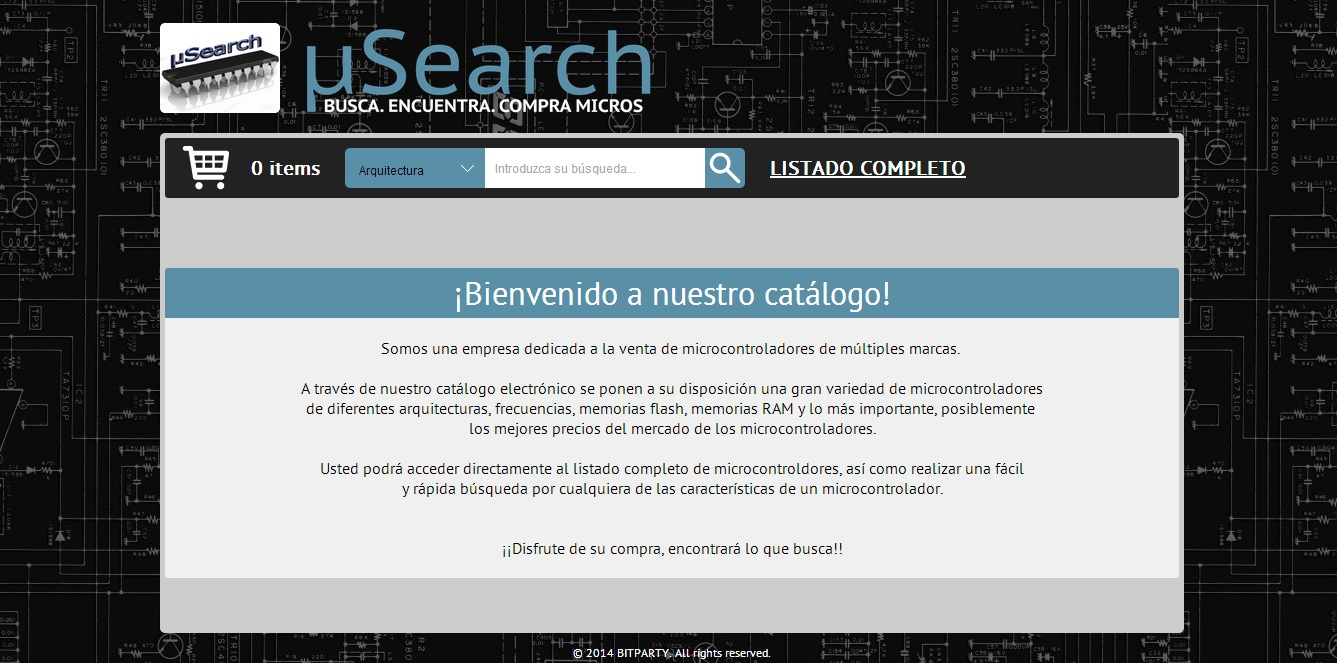
\includegraphics[width=0.85\textwidth]{img/principal_user}
	\caption{Página principal de usuario.}
	\label{fig:principal_usuario}
\end{figure}

Desde esta página, a través de los iconos situados en la cabecera debajo de los logotipos de la web, el usuario puede acceder a:
\begin{itemize}
	\item\textbf{Carrito de la compra:} Redirige al usuario a la página del carrito de la compra.
	
	\item \textbf{Búsqueda:} Desde esta sección, el usuario puede realizar búsquedas sobre el catálogo de microcontroladores en base a cualquiera de sus características (Arquitectura, Frecuencia, Flash, RAM). Se debe seleccionar una de las características de la lista despegable, introducir el texto a buscar y pulsar sobre el icono de búsqueda.
	El usuario será redirigido a una página donde se le mostrará el resultado de la búsqueda.
	
	\item \textbf{Listado Completo:} Redirige al usuario a la página en la que se listan todos los microcontroladores disponibles en el catálogo.
	
\end{itemize}
\newpage

\subsection{Listado completo de microcontroladores}
\paragraph{}En esta página se puede observar el listado completo de todos los microcontroladores existentes en el catálogo electronico y además, en la parte derecha de la especificación de cada microcontrolador, se halla el botón para añadir dicho microcontrolador al carrito de la compra.

\begin{figure}[h!]
	\centering
	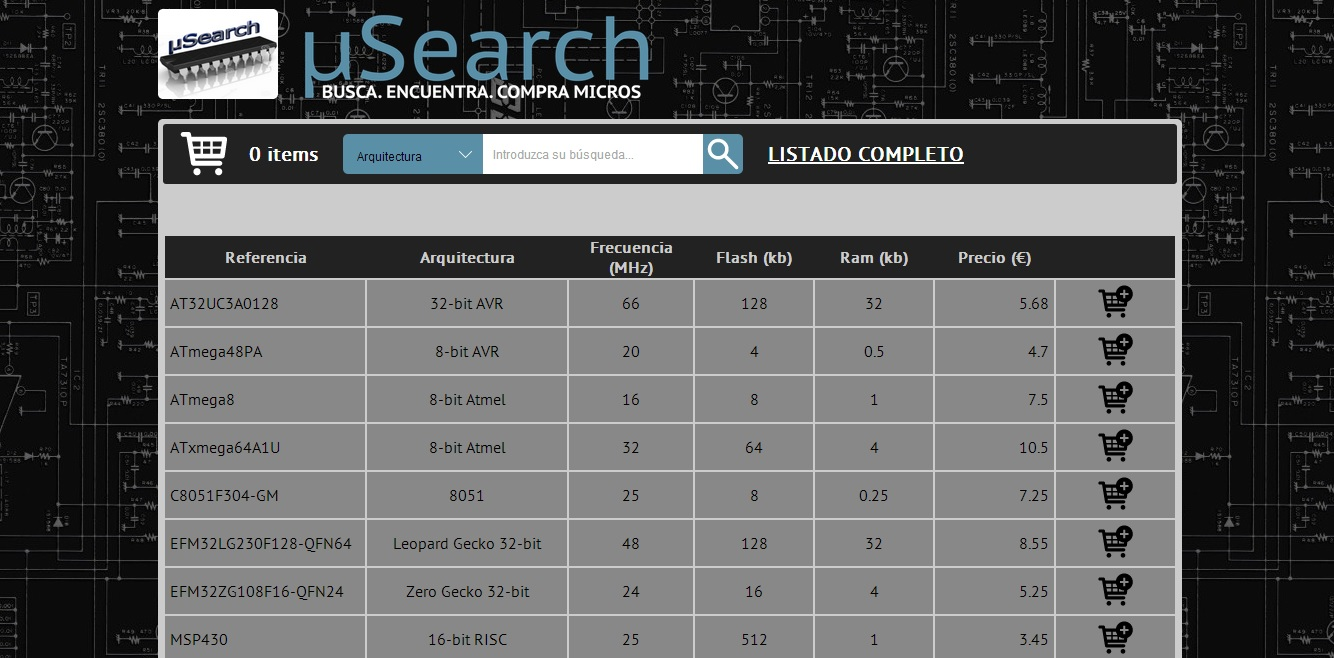
\includegraphics[width=0.85\textwidth]{img/listado_completo_user}
	\caption{Página de listado completo de micro-controladores.}
	\label{fig:listado_completo_user}
\end{figure}

\paragraph{}Desde esta página, a través de los iconos situados en la cabecera debajo de los logotipos de la web, el usuario puede acceder a:

\begin{itemize}
	\item\textbf{Carrito de la compra:} Redirige al usuario a la página del carrito de la compra.
		
	\item \textbf{Búsqueda:} Desde esta sección, el usuario puede realizar búsquedas sobre el catálogo de microcontroladores en base a cualquiera de sus características (Arquitectura, Frecuencia, Flash, RAM). Se debe seleccionar una de las características de la lista despegable, introducir el texto a buscar y pulsar sobre el icono de búsqueda.
	El usuario será redirigido a una página donde se le mostrará el resultado de la búsqueda.
		
	\item \textbf{Listado Completo:} Recarga la página actual.
\end{itemize}
\newpage

\subsection{Listado de resultado de búsqueda}
\paragraph{}En esta página se le muestra al usuario el listado de los microcontroladores existentes en el catálogo electronico que satisfacen los parámetros de la búsqueda que él mismo ha realizado, en base a cualquiera de las características de un microcontrolador. Desde dicho listado el usuario podrá añadir al carrito de la compra los microcontroladores que desee pulsando sobre el botón a la derecha de las especificaciones de cada microcontrolador.

\begin{figure}[h!]
	\centering
	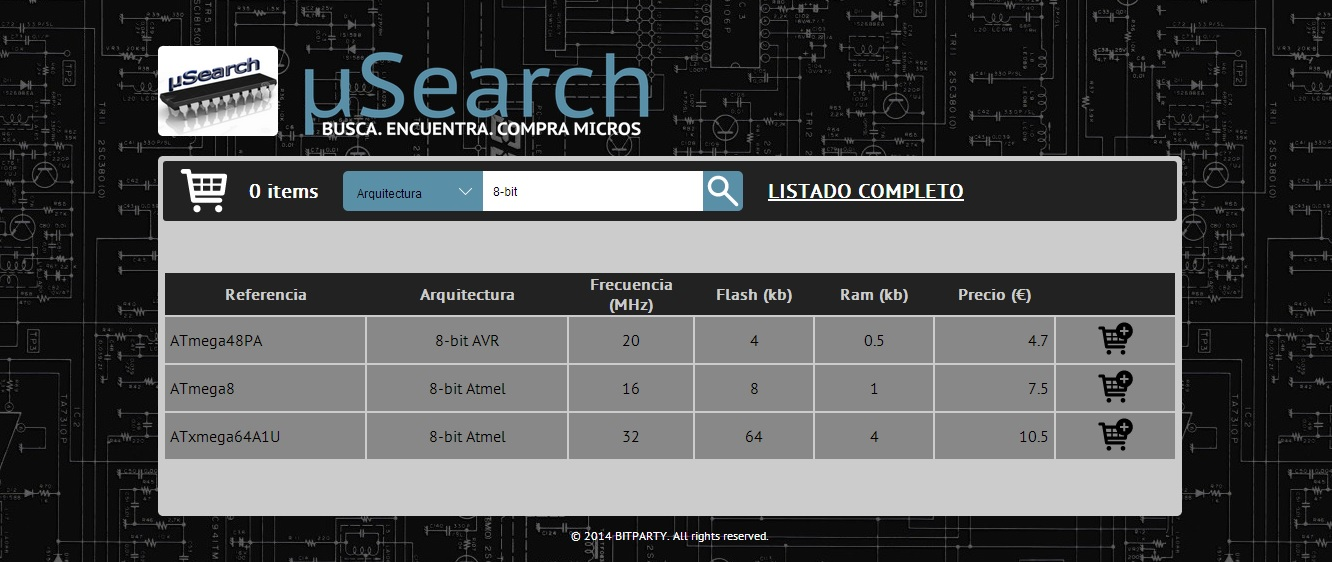
\includegraphics[width=0.85\textwidth]{img/listado_busqueda_user}
	\caption{Página de listado de resultado de búsqueda.}
	\label{fig:listado_busqueda_user}
\end{figure}

\paragraph{}Desde esta página, a través de los iconos situados en la cabecera debajo de los logotipos de la web, el usuario puede acceder a:

\begin{itemize}
	\item\textbf{Carrito de la compra:} Redirige al usuario a la página del carrito de la compra.
	
	\item \textbf{Búsqueda:} Desde esta sección de la cabecera, el usuario puede realizar de nuevo una búsqueda distinta sobre el catálogo de microcontroladores en base a cualquiera de sus características (Arquitectura, Frecuencia, Flash, RAM). Se debe seleccionar una de las características de la lista despegable, introducir el texto a buscar y pulsar sobre el icono de búsqueda.
	El usuario será redirigido a una página donde se le mostrará el resultado de la búsqueda.
		
	\item \textbf{Listado Completo:} Redirige al usuario a la página en la que se listan todos los microcontroladores disponibles en el catálogo.
\end{itemize}
\newpage

\subsection{Carrito de compra}
\paragraph{}En esta página se le muestra al usuario el total de los microcontralodores, tanto en unidades como en precio, que ha ido añadiendo a su carro de la compra durante su visita a la página web $\mu$Search, permitiéndole al usario modificar dichas unidades de cada microcontrolador elegido y finalmente generar un presupuesto o factura.

\begin{figure}[h!]
	\centering
	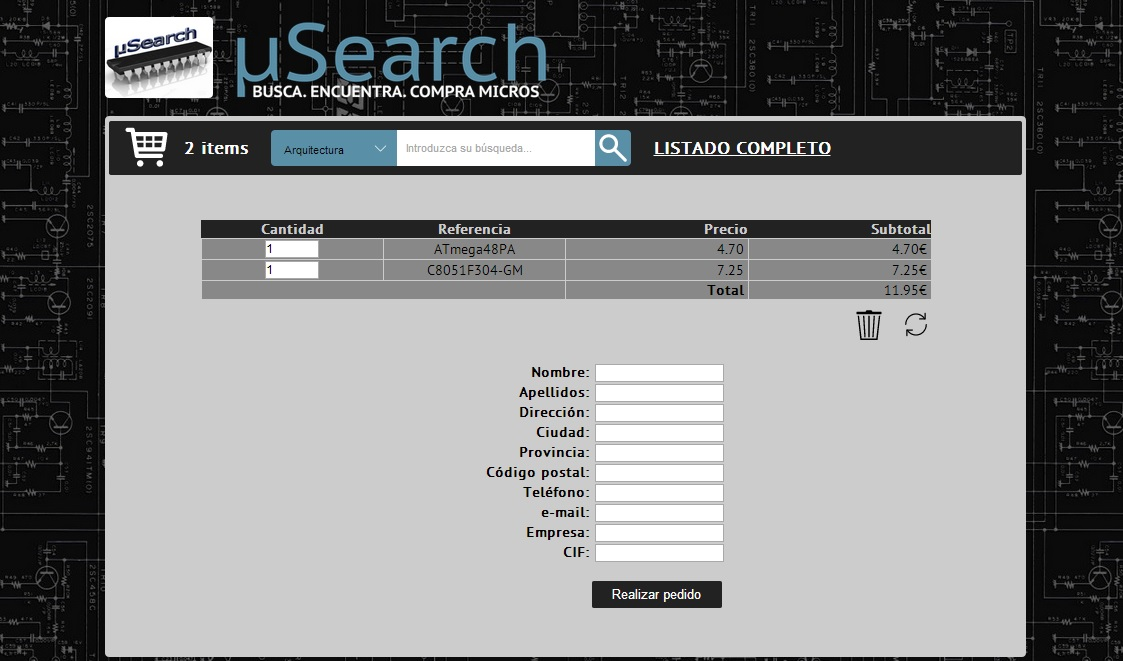
\includegraphics[width=0.75\textwidth]{img/carrito}
	\caption{Carrito de la compra.}
	\label{fig:carrito}
\end{figure}

\paragraph{}Desde esta página, a través de los iconos situados en la cabecera debajo de los logotipos de la web, el usuario puede acceder a:

\begin{itemize}
	\item \textbf{Carrito de la compra:} A su lado, aparece también el número de artículos que han sido introducidos en el mismo, pulsando sobre este icono se vuelve a cargar la página actual. Volver a cargar la página actual puede ser útil en el caso de que se haya modificado la cantidad de uno o varios artículos del carrito y se quiera deshacer estos cambios sin que tengan ningún efecto en el precio final de la compra.

	\item \textbf{Búsqueda:} Desde esta sección de la cabecera, el usuario puede realizar de nuevo una búsqueda distinta sobre el catálogo de microcontroladores en base a cualquiera de sus características (Arquitectura, Frecuencia, Flash, RAM). Se debe seleccionar una de las características de la lista despegable, introducir el texto a buscar y pulsar sobre el icono de búsqueda.
	El usuario será redirigido a una página donde se le mostrará el resultado de la búsqueda.

	\item \textbf{Listado Completo:} Redirige al usuario a la página en la que se listan todos los microcontroladores disponibles en el catálogo.
\end{itemize}

A continuación, se encuentra en forma de tabla el listado de los microcontroladores que el usuario ha ido añadiendo al carrito de la compra. Este listado, esta compuesto por cuatro columnas: 
\begin{itemize}
	\item \textbf{Cantidad:} La cantidad de unidades de cada elemento añadido al carrito de la compra es un campo modificable que permite	solicitar más o menos unidades de ese elemento. Para que estos cambios tengan efecto es necesario actualizar el listado como se explica en el apartado siguiente. Si el usuario pulsa la tecla \textit{Enter} del teclado, teniendo todavía activo el campo de la cantidad de un elemento, también implica aceptar los cambios realizados hasta el momento.
	
	\item \textbf{Referencia:} Es el código del fabricante que identifica a cada elemento del catálogo, cada microcontrolador
	tiene una referencia única.
	
	\item \textbf{Precio:} Es el precio que tiene una unidad de un microcontrolador específico.

	\item \textbf{Subtotal:} Es el resultado de multiplicar el número de unidades solicitadas de un microcontrolador por el precio que tiene cada unidad. Hay tantos subtotales como elementos en el carrito de la compra.
\end{itemize}

Debajo del listado de los elementos del carrito de la compra, se encuentran dos botones que pueden tener efecto sobre todos los microcontroladores solicitados:
\begin{itemize}
	\item \textbf{Actualizar:}  Este botón hay que pulsarlo después de modificar una o varias cantidades de los elementos del 
	carrito de la compra. Es el que permite que dichos cambios tengan efecto. Se puede observar cómo cambia el precio total de la compra.
	Además, si alguna nueva cantidad tiene un valor de 0, el elemento que tenga dicha cantidad será eliminado del carrito de la compra.
	
	\item \textbf{Vaciar:}  Pulsando sobre este botón se vacía completamente el carrito de la compra.
\end{itemize}

\paragraph{}Antes de finalizar el pedido, hay disponible un formulario que el cliente debe rellenar con sus datos de contacto para poder generar correctamente la factura asociada al pedido que se quiere realizar. Todos los campos son obligatorios excepto el nombre y CIF de la empresa.

\paragraph{}Finalmente, una vez que el cliente ha revisado que todos los datos relativos al pedido (cantidades, referencias, precios, datos personales, etc.) son correctos hay que pulsar sobre el botón \textbf{\textit{''Realizar Pedido''}} para que el sistema genere la factura asociada a dicho pedido.
\newpage

\subsection{Generación de pedido}
\paragraph{}Tras haber solicitado el presupuesto mediante el botón \textit{\textbf{''Realizar Pedido''}}, el usuario es redirigido automáticamente a la función de imprimir de su navegador para poder imprimir el pedido que se genera en formato PDF. En el que se muestra toda la información relativa al pedido que se acaba de realizar. Un pedido está compuesto por los siguientes elementos:

\begin{itemize}
	\item \textbf{Tabla de artículos solicitados:} En esta tabla se refleja el número de unidades de cada artículo, las referencias, el precio por unidad de cada uno, el precio subtotal para cada referencia y el precio final del pedido.
	
	\item \textbf{Datos del cliente:} Listado con los datos introducidos por el cliente que permiten tanto identificar al cliente como contactar con él si fuese necesario.
\end{itemize}

\begin{figure}[h!]
	\centering
	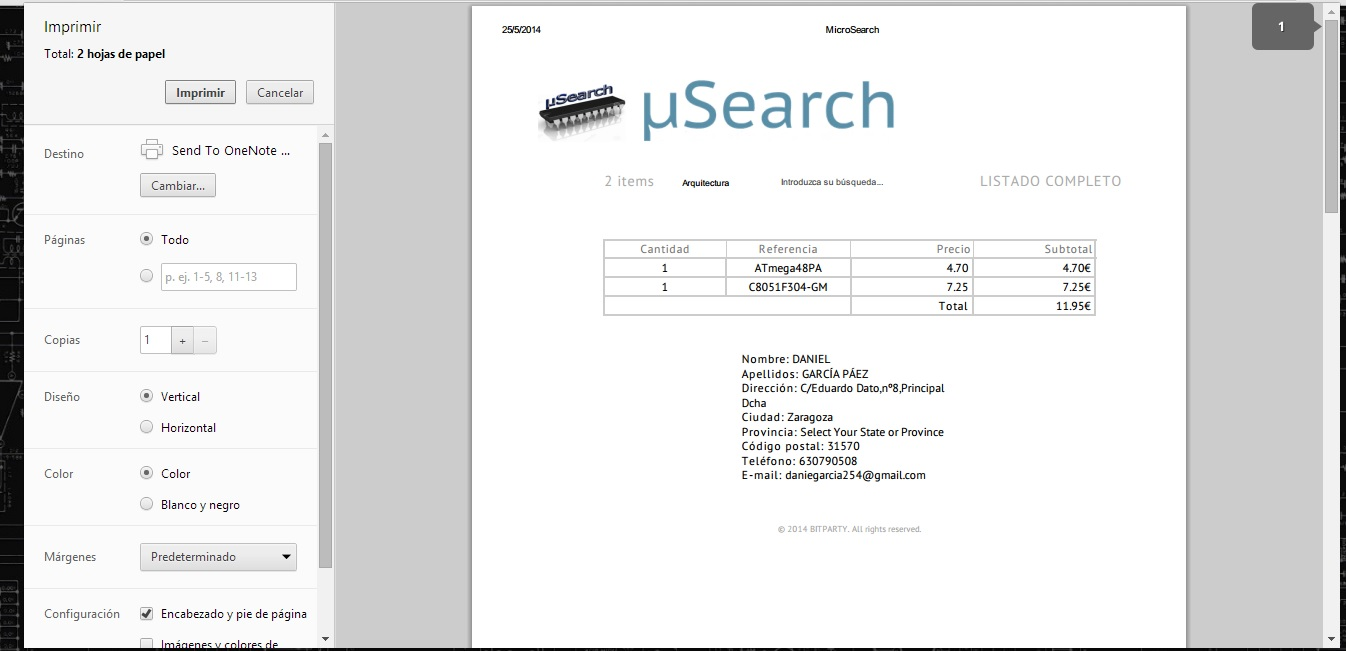
\includegraphics[width=0.85\textwidth]{img/pedido}
	\caption{Pedido generado en PDF.}
	\label{fig:pedido}
\end{figure}

\paragraph{} Tras imprimir el pedido, o cancelar su impresión, al usaurio se le muestra un mensaje de agradecimiento por su compra; pudiendo de nuevo navegar libremente por el catálogo y realizar más pedidos.
\newpage


%----------------------------------------------------------------------------------------
% 3. GUÍA PARA EL ADMINISTRADOR
% 3.1 PÁGINA PRINCIPAL
% 3.2 LISTADO COMPLETO DE MICROCONTROLADORES
% 3.3 LISTADO DE RESULTADO DE BÚSQUEDA
% 3.4 AÑADIR MICROCONTROLADOR
% 3.5 EDITAR MICROCONTROLADOR
% 3.6 ELIMINAR MICROCONTROLADOR
%----------------------------------------------------------------------------------------
\section{Guía para el administrador}
\paragraph{}Se presenta aquí la guía para el administrador del catálogo electrónico de microcontroladores $\mu$Search. El administrador tiene diferentes funcionalidades a las del usuario común, resaltando las de añadir, editar y eliminar microcontroladores de la base de datos.

\paragraph{}Así pues, a través de los siguientes apartados se guía al administrador a través del proceso que ha de seguir para un uso correcto y eficiente de la aplicación web $\mu$Search.

\paragraph{}\underline{\textbf{NOTA:}} Todas las páginas del catálogo electrónico a través de las que navegará el usuario contienen en su parte superior izquierda tanto el logo como el título de la página. Siempre \textit{clickando} sobre cualquiera de los dos el usuario será redirigido a la página principal de administración del catálogo electrónico.
\newpage

\subsection{Página principal}
\paragraph{}Esta es la página principal o de inicio de la aplicación web $\mu$Search para el administrador de la misma. A esta página de inicio, el administrador será siempre redirigido cuando pulse en cualquiera de los dos logotipos de la cabecera de la página.

\paragraph{}Se le muestra al administrador un mensaje de bienvenida y una breve descripción las funcionalidades que tiene disponibles como administrador de la aplicación web.

\begin{figure}[h!]
	\centering
	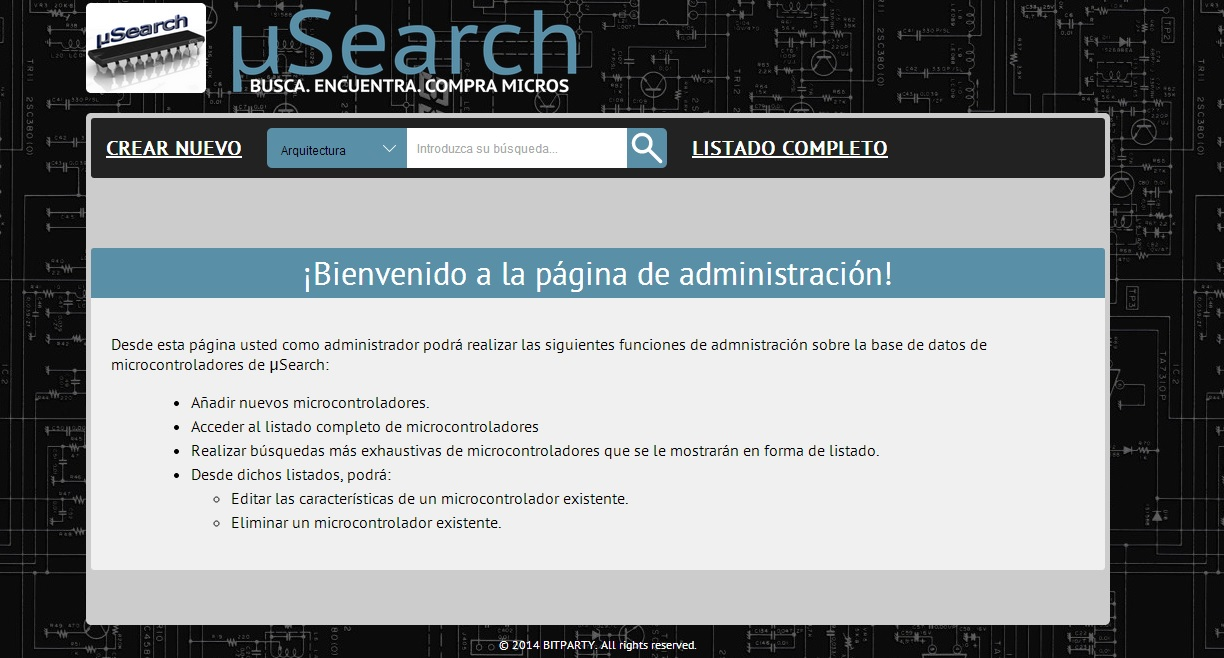
\includegraphics[width=0.85\textwidth]{img/principal_admin}
	\caption{Página principal de administración.}
	\label{fig:principal_admin}
\end{figure}

Desde esta página, a través de los iconos situados en la cabecera debajo de los logotipos de la web, el administrador puede acceder a:
\begin{itemize}
	
	\item \textbf{Crear Nuevo:} Redirige al administrador a la página para añadir un nuevo microcontrolador al catálogo electrónico.
	
	\item \textbf{Búsqueda:} Desde esta sección, el administrador puede realizar búsquedas sobre el catálogo de microcontroladores en base a cualquiera de sus características (Arquitectura, Frecuencia, Flash, RAM). Se debe seleccionar una de las características de la lista despegable, introducir el texto a buscar y pulsar sobre el icono de búsqueda.
	El usuario será redirigido a una página donde se le mostrará el resultado de la búsqueda.
	
	\item \textbf{Listado Completo:} Redirige al administrador a la página en la que se listan todos los microcontroladores disponibles en el catálogo.
	
\end{itemize}
\newpage

\subsection{Listado completo de microcontroladores}
\paragraph{}En esta página se puede observar el listado completo de todos los microcontroladores existentes en el catálogo electronico. En la parte derecha de la tabla, tras la especificación de cada microcontrolador, se hallan los siguientes botones:
\begin{itemize}
	\item \textbf{Editar:} Redirige al administrador a la página para editar la especificación y características de dicho microcontrolador.
	\item \textbf{Eliminar:} Elimina el microcontrolador de la base de datos del catálogo electrónico, recargando la página con el nuevo listado actualizado.
\end{itemize}

\begin{figure}[h!]
	\centering
	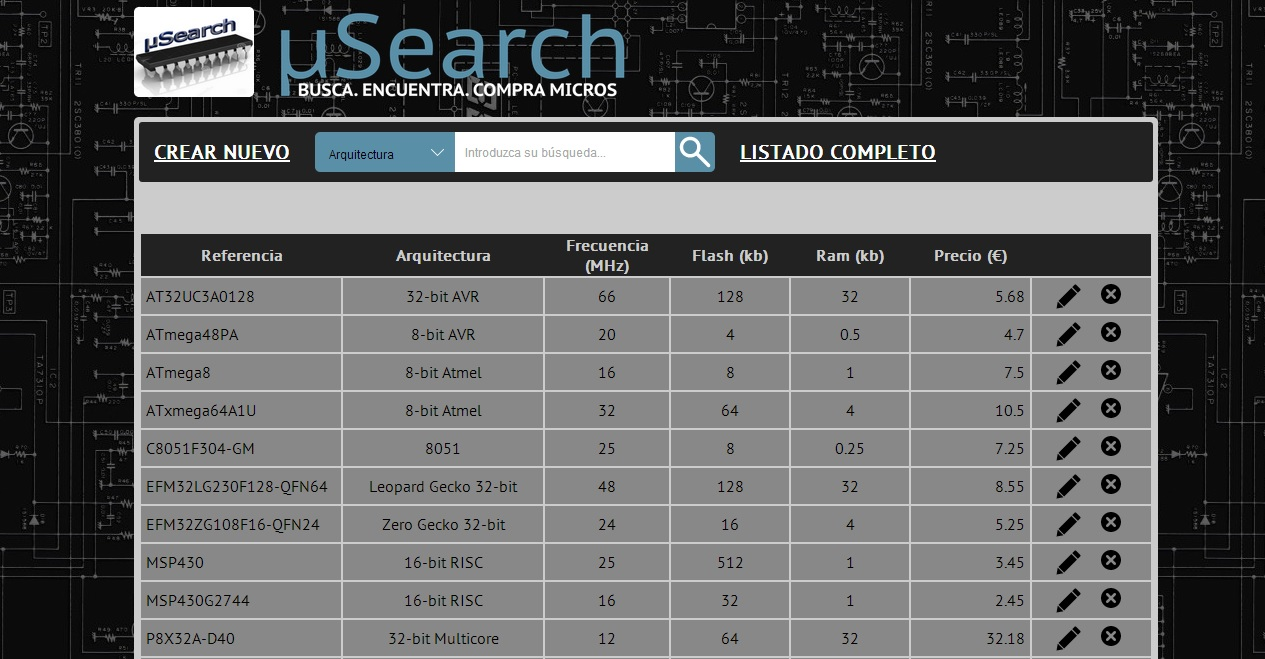
\includegraphics[width=0.80\textwidth]{img/listado_completo_admin}
	\caption{Página de listado completo de micro-controladores.}
	\label{fig:listado_completo_admin}
\end{figure}

\paragraph{}Desde esta página, a través de los iconos situados en la cabecera debajo de los logotipos de la web, el administrador puede acceder a:

\begin{itemize}
	
	\item \textbf{Crear Nuevo:} Redirige al administrador a la página para añadir un nuevo microcontrolador al catálogo electrónico.
		
	\item \textbf{Búsqueda:} Desde esta sección, el administrador puede realizar búsquedas sobre el catálogo de microcontroladores en base a cualquiera de sus características (Arquitectura, Frecuencia, Flash, RAM). Se debe seleccionar una de las características de la lista despegable, introducir el texto a buscar y pulsar sobre el icono de búsqueda.
	El usuario será redirigido a una página donde se le mostrará el resultado de la búsqueda.
			
	\item \textbf{Listado Completo:} Recarga la página actual.
\end{itemize}
\newpage

\subsection{Listado de resultado de búsqueda}
\paragraph{}En esta página se le muestra al administrador el listado de los microcontroladores existentes en el catálogo electronico que satisfacen los parámetros de la búsqueda que él mismo ha realizado. El listado se muestra en forma de tabla, un microcontrolador por fila, proporcionando información de cada una de sus caracterísiticas. En la parte derecha de la especificación de cada microcontrolador, se hallan los siguientes botones:
\begin{itemize}
	\item \textbf{Editar:} Redirige al administrador a la página para editar la especificación y características de dicho microcontrolador.
	\item \textbf{Eliminar:} Elimina el microcontrolador de la base de datos del catálogo electrónico, recargando la página con el nuevo listado actualizado.
\end{itemize}

\begin{figure}[h!]
	\centering
	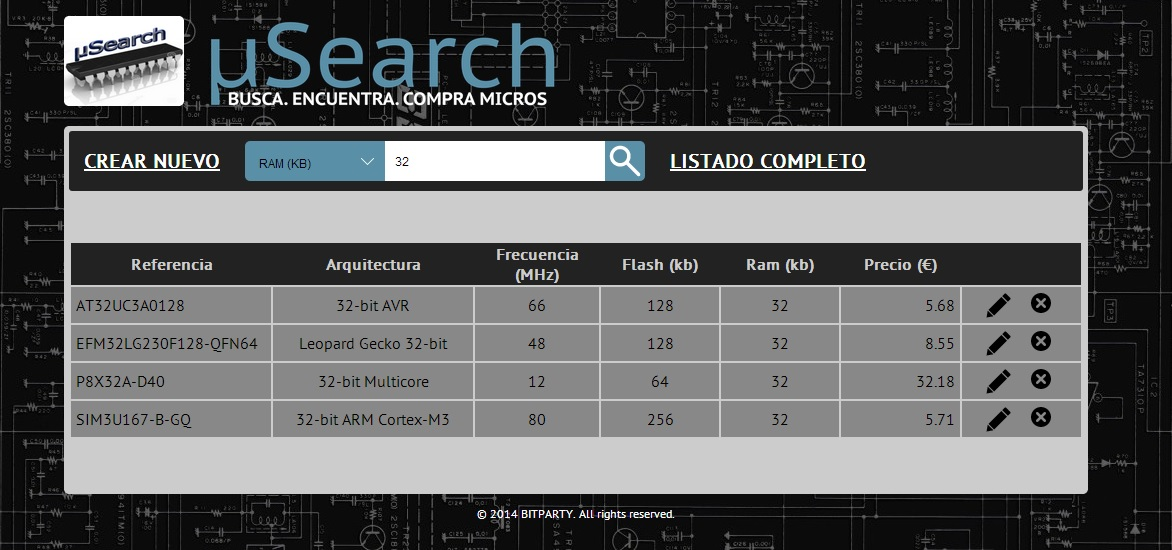
\includegraphics[width=0.70\textwidth]{img/listado_busqueda_admin}
	\caption{Página de listado de resultado de búsqueda.}
	\label{fig:listado_busqueda_admin}
\end{figure}

\paragraph{}Desde esta página, a través de los iconos situados en la cabecera debajo de los logotipos de la web, el administrador puede acceder a:

\begin{itemize}
	\item \textbf{Crear Nuevo:} Redirige al administrador a la página para añadir un nuevo microcontrolador al catálogo electrónico.

	\item \textbf{Búsqueda:} Desde esta sección de la cabecera, el administrador puede realizar de nuevo una búsqueda sobre el catálogo de microcontroladores en base a cualquiera de sus características (Arquitectura, Frecuencia, Flash, RAM). Se debe seleccionar una de las características de la lista despegable, introducir el texto a buscar y pulsar sobre el icono de búsqueda.
	El usuario será redirigido a una página donde se le mostrará el resultado de la búsqueda.
			
	\item \textbf{Listado Completo:} Redirige al administrador a la página en la que se listan todos los microcontroladores disponibles en el catálogo.
\end{itemize}
\newpage

\subsection{Añadir microcontrolador}
\paragraph{} Esta es la página para añadir nuevos elementos en la base de datos de una manera sencilla. En ella aparecen se le presenta al administrador un formulario con los diferentes campos a rellenar de los microcontroladores que son, uno por característica: \textbf{Referencia}, \textbf{Arquitectura}, \textbf{Frecuencia(MHz)}, \textbf{Memoria Flash(KB)}, \textbf{Memoria RAM(KB)} y \textbf{precio (\euro)}.

\paragraph{} Al rellenar todos los campos y pulsar sobre el botón situado a la derecha se añade el elemento a la base de datos y automáticamente se redirigirá al administrador a la página de listado completo, con el nuevo microcontrolador ya incluido en la lista.

\begin{figure}[h!]
	\centering
	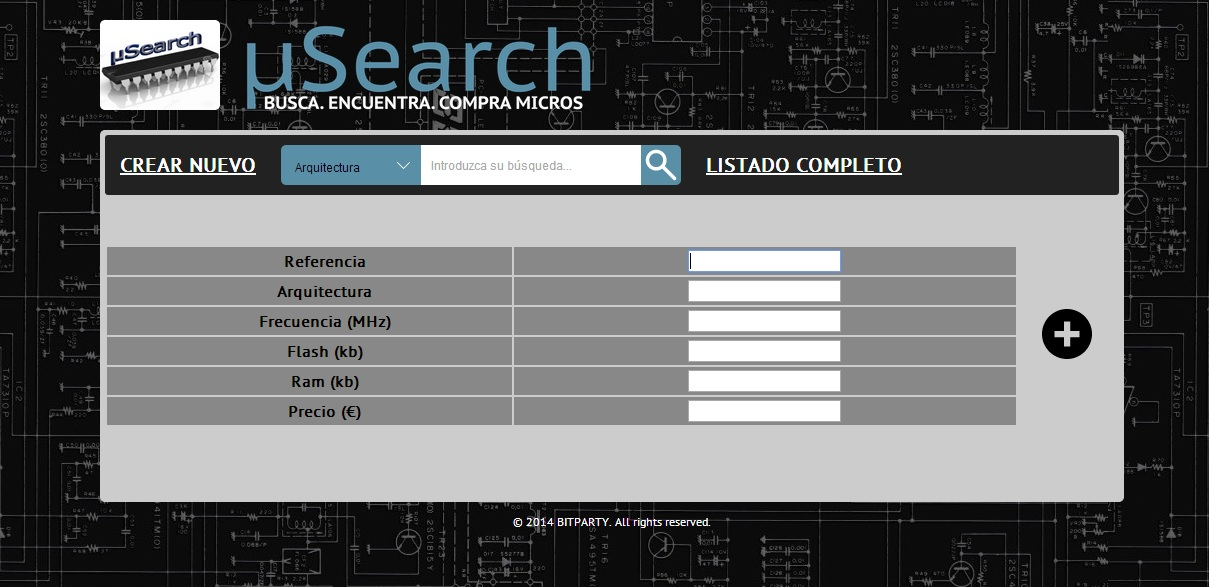
\includegraphics[width=0.75\textwidth]{img/anyadir}
	\caption{Página para añadir un nuevo micro-controlador.}
	\label{fig:anyadir}
\end{figure}

\paragraph{}Además, desde esta página, a través de los iconos situados en la cabecera debajo de los logotipos de la web, el administrador puede acceder a:

\begin{itemize}
	
	\item \textbf{Crear Nuevo:} Recarga la página actual de creación de un nuevo microcontrolador. El formulario actual no se guarda al recargar la página.

	\item \textbf{Búsqueda:} Desde esta sección, el administrador puede realizar búsquedas sobre el catálogo de microcontroladores en base a cualquiera de sus características (Arquitectura, Frecuencia, Flash, RAM). Se debe seleccionar una de las características de la lista despegable, introducir el texto a buscar y pulsar sobre el icono de búsqueda.
	El usuario será redirigido a una página donde se le mostrará el resultado de la búsqueda.
			
	\item \textbf{Listado Completo:} Redirige al administrador a la página en la que se listan todos los microcontroladores disponibles en el catálogo.
\end{itemize}
\newpage

\subsection{Editar microcontrolador}
\paragraph{} Esta es la página para modificar elementos en la base de datos de una manera sencilla. Aquí se muestra al administrador un formulario con un campo por característica del microcontrolador, con la información actual sobre el mismo ya cargada, y que el administrador puede modificar a su gusto. El campo \textbf{''Referencia''} no será editable.

\paragraph{} Al pulsar el botón situado a la derecha se modifica el elemento en la base de datos y automáticamente se redirigirá al administrador a la página de listado completo, con el nuevo microcontrolador ya incluido en la lista.

\begin{figure}[h!]
	\centering
	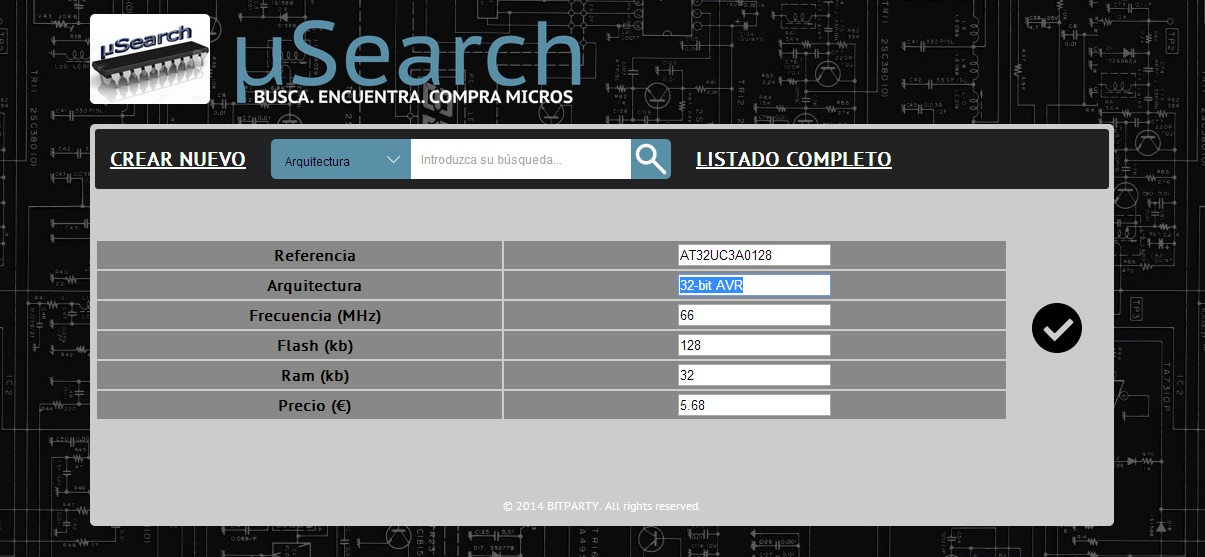
\includegraphics[width=0.75\textwidth]{img/editar}
	\caption{Página para modificar un micro-controlador.}
	\label{fig:editar}
\end{figure}

\paragraph{}Además, desde esta página de edición, a través de los iconos situados en la cabecera debajo de los logotipos de la web, el administrador puede acceder a:

\begin{itemize}
	\item \textbf{Crear Nuevo:} Redirige al administrador a la página para añadir un nuevo microcontrolador al catálogo electrónico.

	\item \textbf{Búsqueda:} Desde esta sección, el administrador puede realizar búsquedas sobre el catálogo de microcontroladores en base a cualquiera de sus características (Arquitectura, Frecuencia, Flash, RAM). Se debe seleccionar una de las características de la lista despegable, introducir el texto a buscar y pulsar sobre el icono de búsqueda.
	El administrador será redirigido a una página donde se le mostrará el resultado de la búsqueda.
			
	\item \textbf{Listado Completo:} Redirige al administrador a la página en la que se listan todos los microcontroladores disponibles en el catálogo.
\end{itemize}

\end{document}
